\section{Suppressing the Spiders by using FFT}
We now want to use the knowledge we have gained about the Fourier transformation of different features, especially of features which resemble spiders, to suppress the signal of the spiders. The idea is to manipulate the Fourier transform of the data and then transform the data back via the inverse Fourier transformation.\\
We take the data from HD142527, warp it to the $r$-$\varphi$ plane and correct for the radial intensity drop. For the transformation we choose the radius range such that the object we want to look at is placed in the center. We choose the same radius range as in figure \ref{fig:warped_254_454} namely: $R=254-454$. In order to make sure that the aperture flux of other objects than the spiders, mainly point sources like exoplanets, is conserved we will use the ghost at radius $323$. The ghost is not perfectly in the center of the radius range, but this is not important for our purpose. The only thing which will happen, is that the aperture flux will change a bit when warping the image to the $r$-$\varphi$ plane.\\
Figure \ref{fig:rad0} shows the Fourier transform of the warped and flatten image at different radial frequencies. In contrast to the Fourier transform of the simulated spiders, the signal is not Gaussian anymore, since there are other features on top, like the ghost and the noise.
\begin{figure}[H]
	\centering
		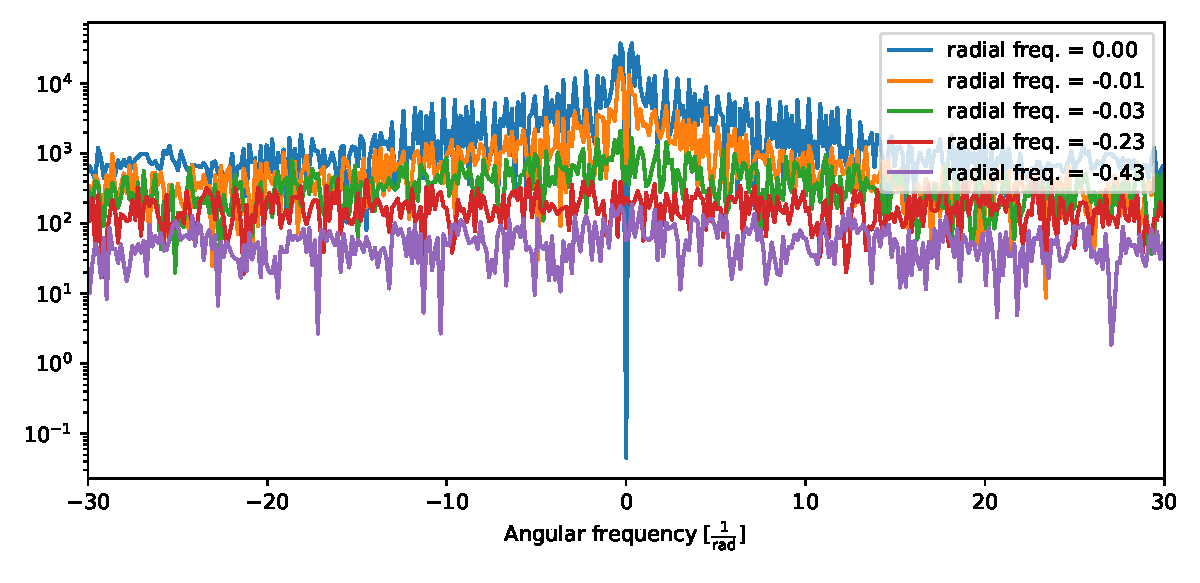
\includegraphics[width=1.0\textwidth]{pics/rad0.pdf}
		\caption{Several horizontal cuts through the frequency plane of the image data shown in figure \ref{fig:HDflatten_R254_R454_-1to1}.}
		\label{fig:rad0}
\end{figure} 
As we saw in section \ref{sec:pointlike} the angular range in which a point-source, Gaussian or PSF, will produce a significant frequency signal is within $[-50, 50] \frac{1}{\mathrm{rad}}$ and the radial range is within $[-0.2, 0.2] \frac{1}{\mathrm{px}}$. Therefore we will suppress everything which is outside of this area by a factor of $1000$. The ghost looses $0.07$ \% of its aperture flux due to this suppression. \\
Instead of suppressing everything outside of this rectangular area, we could also use a filter, i.e. a butterworth filter. This is however fine tuning and can still be changed in the end.\\
As a next step, we want to subtract the frequencies for radial frequency zero, which are caused by the spiders. As we saw in section \ref{sec:gaussian} the spiders produce a signal in the frequency plane, especially for radial frequency equals zero, which is close to a Gaussian. We subtract the same Gaussian from it, as we found from our simulations of the spiders, see figure \ref{fig:simspi_angularfreq}. This can be done without any problems, due to the fact that the resulting image, which we gain after an inverse Fourier transform, is not sensible on the width and the intensity of the Gaussian. What is important for the resulting image is the angular range for which the subtraction is done. Figure \ref{fig:rad0_diffsubwidths} shows the aperture flux of the ghost after the subtraction of a Gaussian at radial frequency zero for different angular frequency ranges around zero (symmetric). The orange line marks the aperture flux of the ghost after the warping and the correction for the radial drop-off, we call it the initial aperture flux. Since it is even an advantage if the aperture flux increases through the procedure, we choose the width with which we get the largest aperture flux, which is the case for $9.7 \frac{1}{\mathrm{rad}}$. This means we subtract the Gaussian in the following angular range: $[-9.7, 9.7] \frac{1}{\mathrm{rad}}$. An increase of the aperture flux is really good, because it means that the spiders are being suppressed without suppressing the ghost. Ghost 2, at which we are looking, is a good indicator for this, because in this image he is situated close to a spider.
\begin{figure}[H]
	\centering
		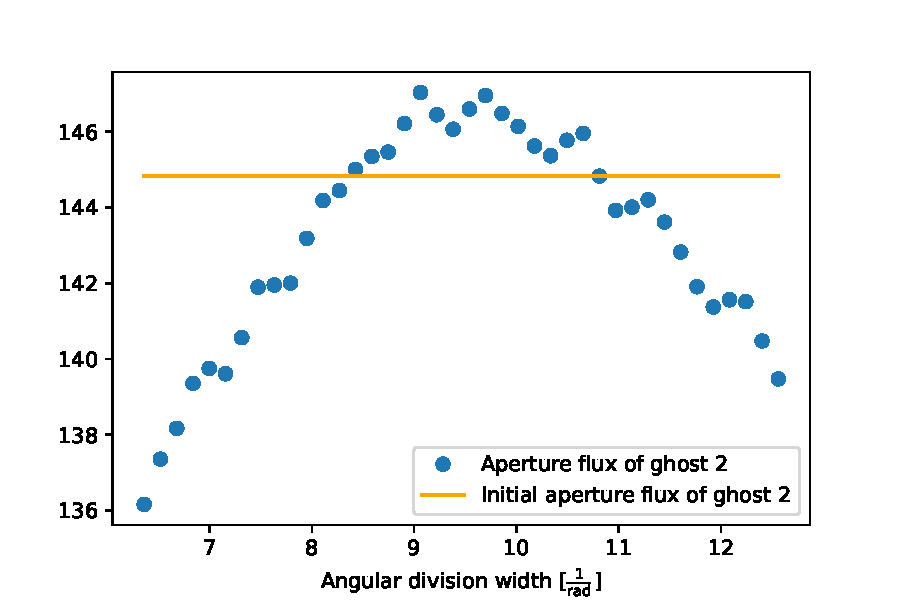
\includegraphics[width=1.0\textwidth]{pics/rad0_diffsubwidths.pdf}
		\caption{For radial frequency zero from the Fourier transform of the image data a Gaussian is subtracted which has its center at angular frequency zero. The Gaussian is not subtracted along the complete angular range, but only for a certain width around zero. We have plotted the aperture flux of ghost 2 for different widths. The width which produces the largest flux is ideal.}
		\label{fig:rad0_diffsubwidths}
\end{figure}
Figure \ref{fig:HDcentralfreq_R254_R454_-1to1} shows the frequency plane of the image after the outer frequencies are suppressed and the Gaussian for radial frequency zero is subtracted. To get back into the $r$-$\varphi$ plane we use the inverse Fourier transformation. The result of this back transformation is also shown in figure \ref{fig:HDcentralfreq_R254_R454_-1to1}. When we compare the image before, figure \ref{fig:HDflatten_R254_R454_-1to1}, and after the Gaussian subtraction we can already observe that the spiders are a lot less bright, especially around the central radius. This is for us the most important region, since this is also the region where the object we are interested in, will be. Also the noise gets weaker and is smoother distributed. \\
From the steps we have made so far the aperture flux increases by $4.30$ \% compared to the initial aperture flux. 
\begin{figure}[H]
	\centering
		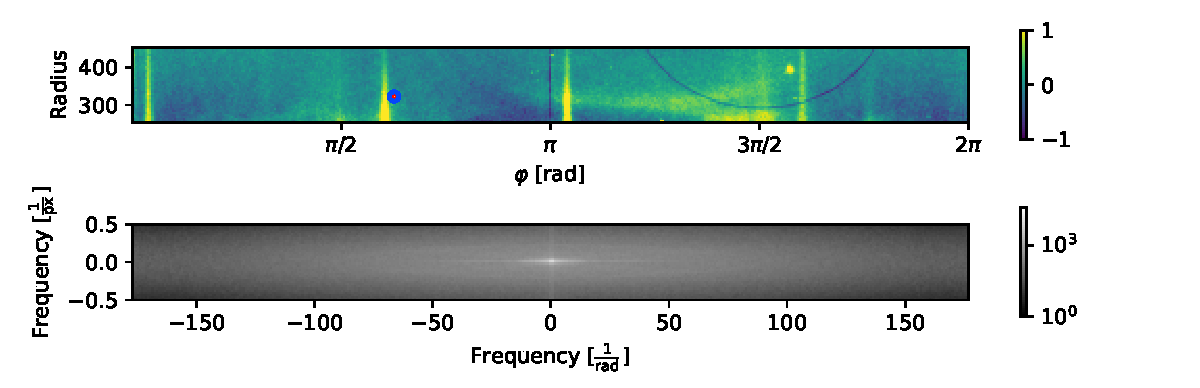
\includegraphics[width=1.0\textwidth]{pics/HDflatten_R254_R454_-1to1.pdf}
		\caption{An image from HD142527 which has been warped to the $r$-$\varphi$ plane and flattened and its Fourier transform.}
		\label{fig:HDflatten_R254_R454_-1to1}
\end{figure}
\begin{figure}[H]
	\centering
		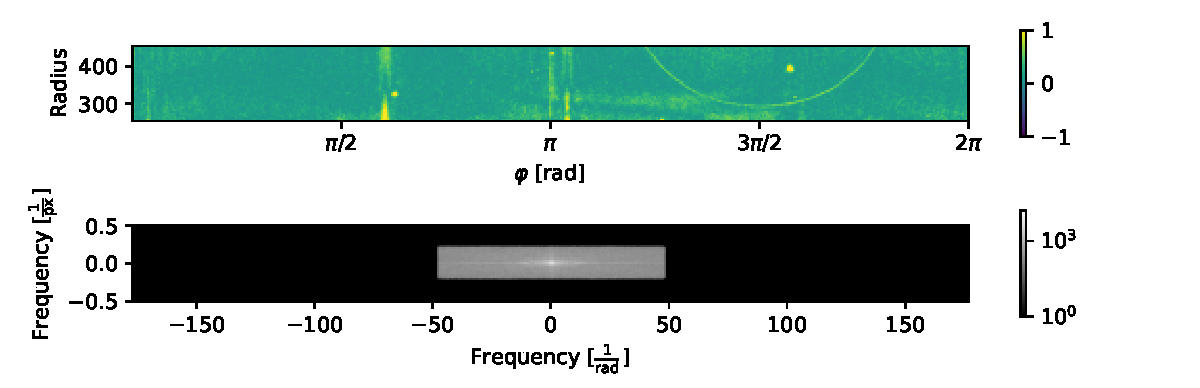
\includegraphics[width=1.0\textwidth]{pics/HDcentralfreq_R254_R454_-1to1.pdf}
		\caption{The outer frequencies of the Fourier transform of figure \ref{fig:HDflatten_R254_R454_-1to1} are suppressed and a Gaussian is subtracted from the central frequencies at radial frequency zero, which is shown at the bottom. By using inverse Fourier transformation the image at the top can be found.}
		\label{fig:HDcentralfreq_R254_R454_-1to1}
\end{figure}

As we saw during the simulation of the spiders, not only the frequencies at radial frequency zero have non-zero values, but there is also an extension into the radial frequencies which are unequal to zero. In the previous we will suppress the frequencies caused by the spiders, also in this regime.